\newpage

\section{Runtime view}
\label{RuntimeView}
    
In this section will be analysed the runtime view of the system. It shows, more in detail, how the system works in every use case, presenting the interaction between the internal components, discussed above in the section \ref{ComponentView}.

\subsection{Data4Help}

Concerning Data4Help, the main functionalities taken into account are: the registration procedure, the log in procedure, the subscription for a request, the unsubscription and both single user request and multiple users request.

\subsubsection{Registration and Login}
In the diagram below is presented the workflow of the application during the registration and the log in. This diagram shows the case of registration and the log in of an individual to the system. However, the client type is not specified because the behaviour is the same also in case of Third Party.
The main component is the Account Manager, that inserts in the database the data of new users and, communicating with the Login and Registration Manager, checks the credential after a log in request.

    
\begin{figure}[H]
    \centering
    \makebox[\textwidth][c]{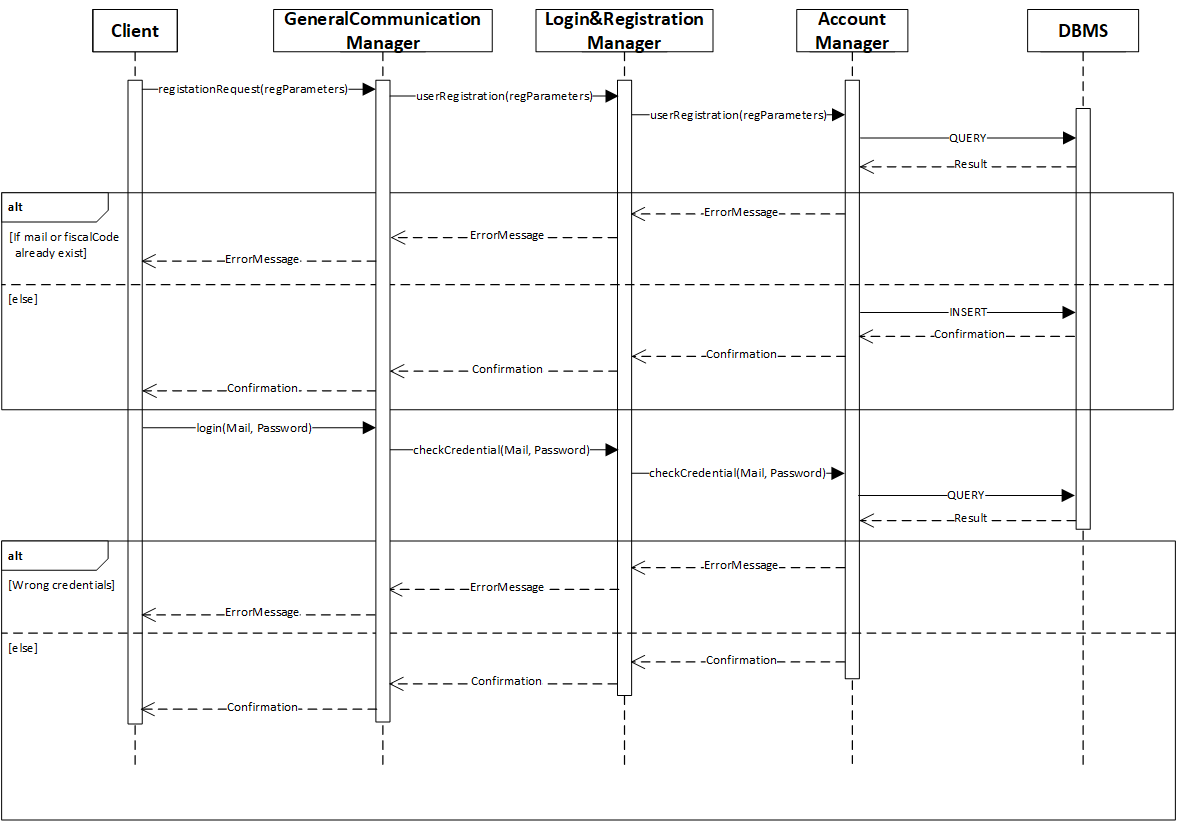
\includegraphics[scale=0.60]{pictures/Registration&LoginSequenceDiagram.png}}
    \caption{Registration and Login sequence diagram}
    \label{fig:log&regDiagram}
\end{figure}

\subsubsection{Single User data request}
This diagram analyses the single request made by a Third-party to a specific registered Individual.
The request is taken by the Request Manager, that verifies the correctness of the demanded fiscal code. Then, in case of positive match, the responsibility passes to the Privacy Manager that, through the General Communication Manager, informs the user and collects his/her consents.
After this procedure the data are sent to the requester and the Account Manager saves the request's details in the database, in order to make the data available to the Third-party also at a later time.

\begin{figure}[H]
    \centering
    \makebox[\textwidth][c]{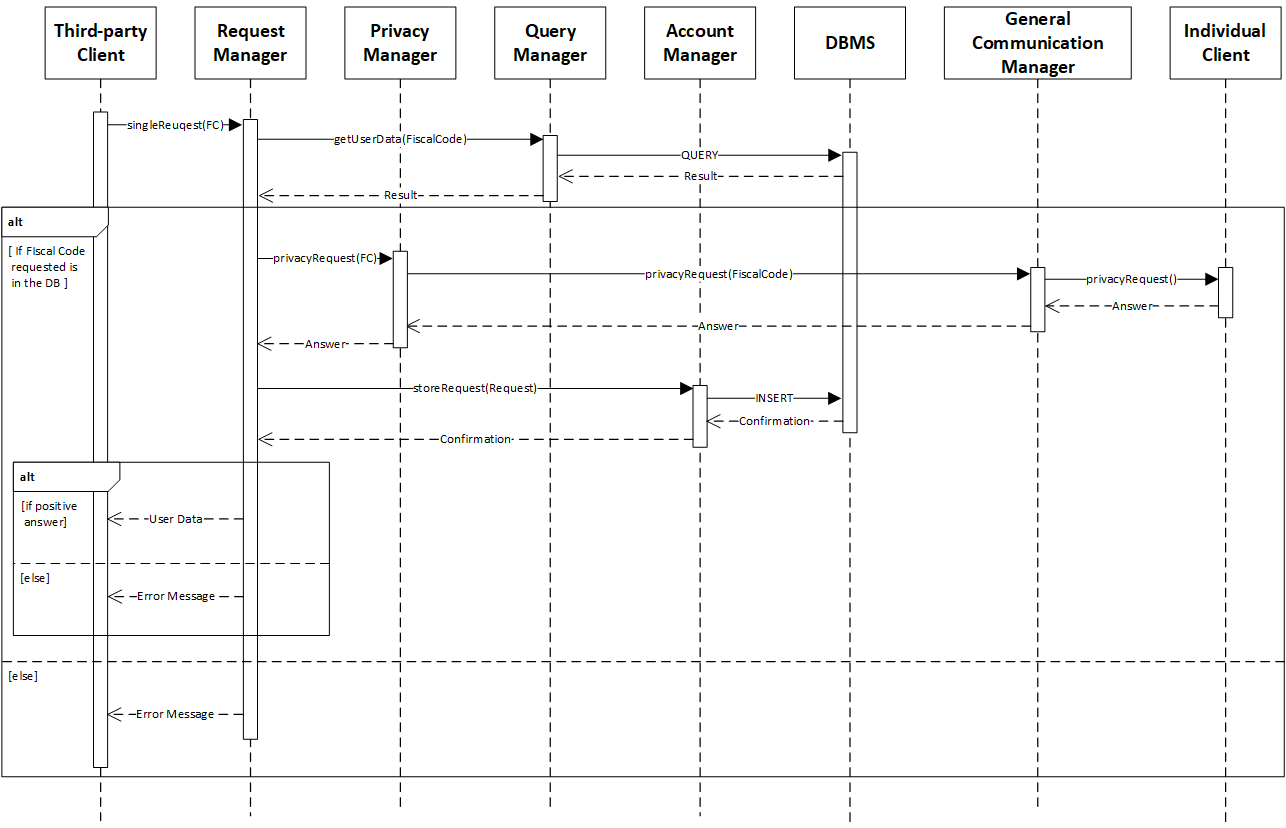
\includegraphics[scale=0.60]{pictures/SingleUserDataRequest.png}}
    \caption{Single user request sequence diagram}
    \label{fig:log&regDiagram}
\end{figure}

\subsubsection{Aggregated data request}
For an aggregated data request the procedure is very similar to the previous one, indeed there are the same actors, except for the Privacy Manager, and the roles taken by them are mostly the same.
However, as already discussed in the RASD, the system can not send the data that match with the filters received, if they belong to a little amount of people. Therefore, the Request Manager, before sending them, has to verify if the corresponding number of people is greater than 1000, then, in case of positive answer, it can send them to the Third-party.

\begin{figure}[H]
    \centering
    \makebox[\textwidth][c]{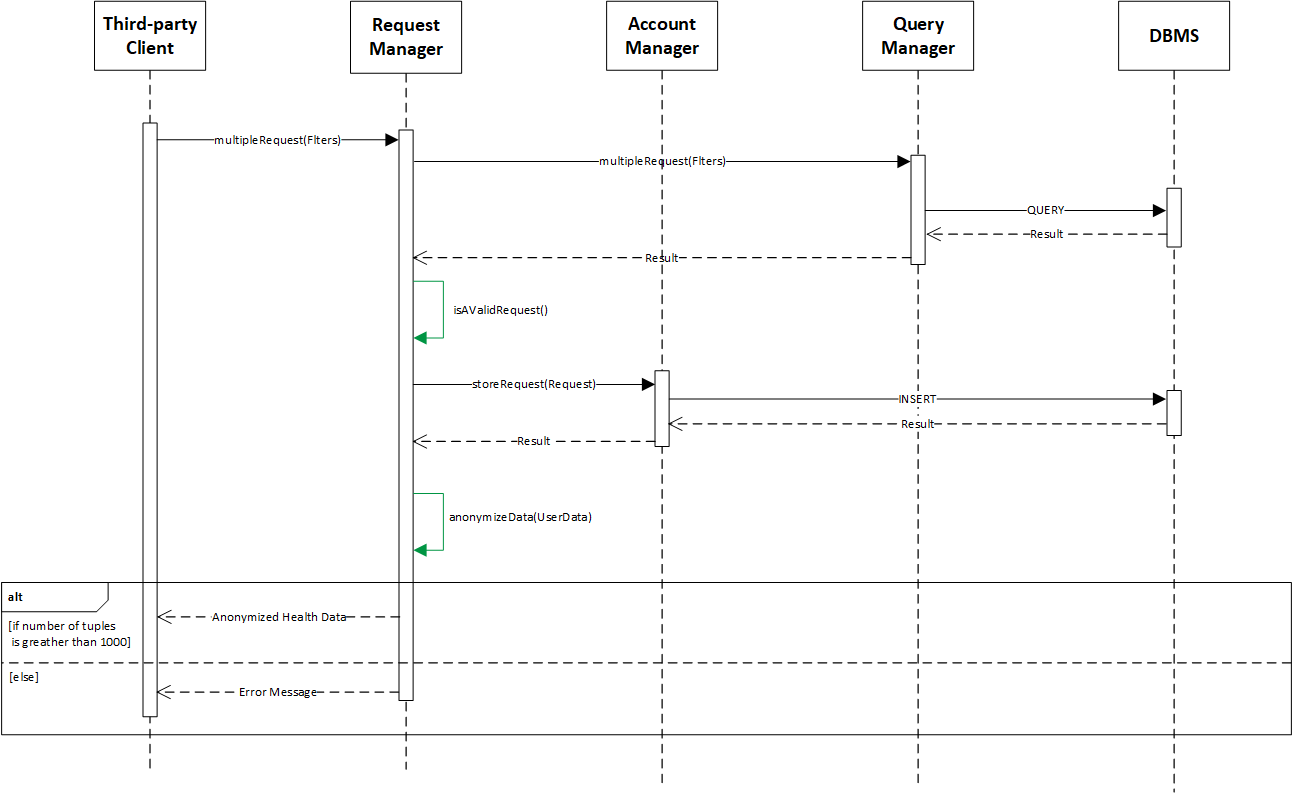
\includegraphics[scale=0.60]{pictures/MultipleUserDataRequest.png}}
    \caption{Aggregated data request sequence diagram}
    \label{fig:log&regDiagram}
\end{figure}

\subsubsection{Single User Data Subscription and Unsubscription}
The following diagram shows the behaviour of the system in case of single request with subscription and the consecutive unsubscription to it.
In the first part is analysed how the system reacts in case of subscription request. The Request Manager passes the control to a subcomponent, the Subscription Manager, that generates a new instance to manage the subscription in its entire life. Then the flow is the same of a normal single request, the first data collected are sent immediately to the Third-party, with the only difference that, when the Account Manager stores the request details, it includes also the information about the subscription.
On the other hand, the part in the bottom describes what happened when, after some time, the user wants to end the subscription. The Account Manager receives the request, it deletes the subscription in the database and informs the Subscription Manager, that in turn deletes the instance related to that subscription.
Furthermore, it notifies with a confirmation the user and sends a notification to the Third-party connected to it.
The same happens also in case of opposite situation, when a Third-party wants to end a subscription. In that case, the confirmation is sent to it and the notification to the corresponding Individual.

\begin{figure}[H]
    \centering
    \makebox[\textwidth][c]{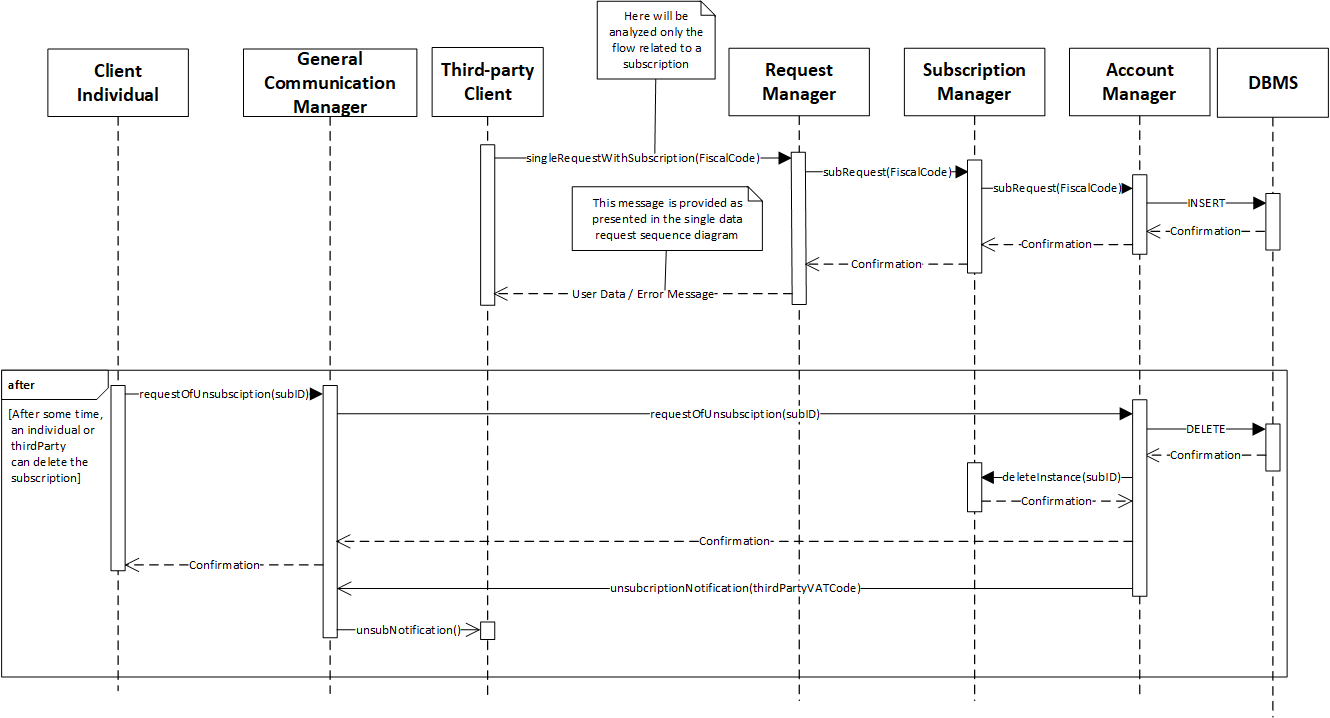
\includegraphics[scale=0.60]{pictures/SingleUserDataSubscription&Unsubscription.png}}
    \caption{Subscription and Unsubscription request sequence diagram}
    \label{fig:log&regDiagram}
\end{figure}

\subsubsection{Group search unsubscription}
In case of unsubscription for a group search, the system manages the request in an easier way compered to the single request unsubscription. Since no user is directly connected, the Account Manager just deletes the information on the database and informs the Subscription Manager, that behaves in the same way respect to the single request unsubscription.
At the end the confirmation is sent only to the Third-party that made the request.

\begin{figure}[H]
    \centering
    \makebox[\textwidth][c]{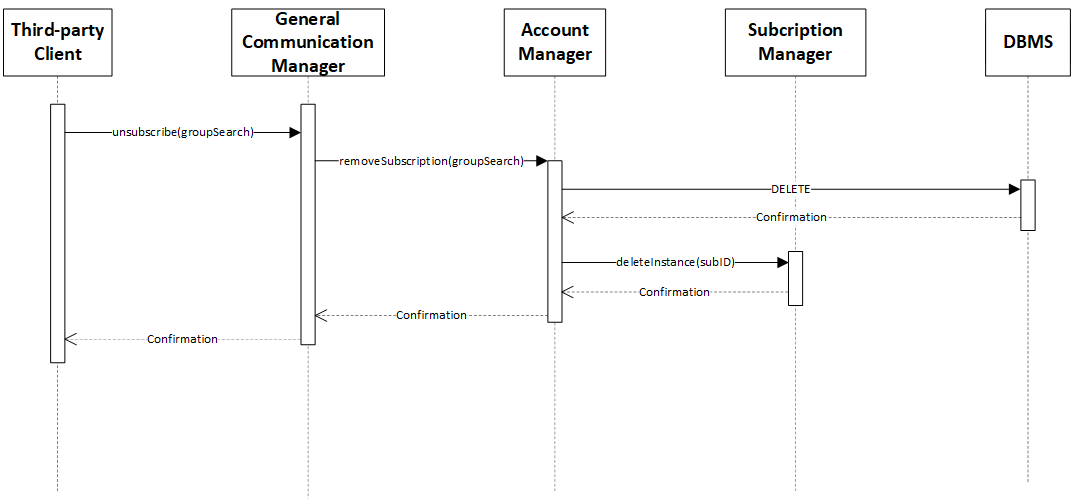
\includegraphics[scale=0.60]{pictures/GroupSearchUnsubscription.png}}
    \caption{Group search unsubscription sequence diagram}
    \label{fig:log&regDiagram}
\end{figure}

\subsubsection{Data dispatching during subscription}
The next diagram displays how the Subscription Manager carries out its work during the subscription. Until the end of the subscription, it periodically extracts the data from the database thanks to the Query Manager and it sends them to the Third-party subscribed. The only important thing to highlight is that with Subscription Manager in the diagram, it is intended the instance correlated to a specific subscription, because there isn't a component who manages all the subscription but, as earlier discussed, each subscription is managed by a different instance.
In the diagram is presented the case of single request subscription, but the same takes place also for a group request subscription.

\begin{figure}[H]
    \centering
    \makebox[\textwidth][c]{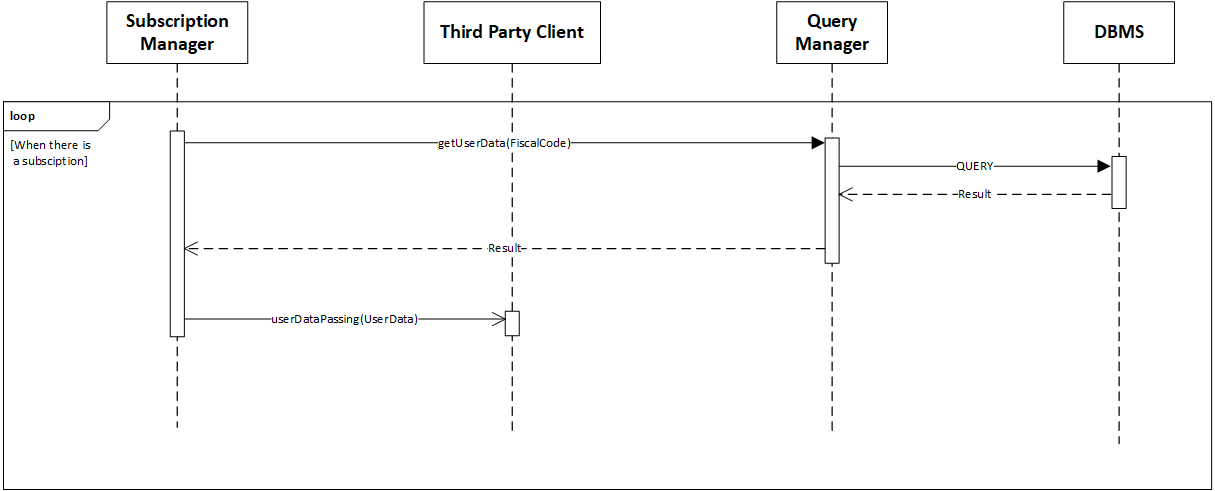
\includegraphics[scale=0.60]{pictures/SendDataDuringSingleSubscription.png}}
    \caption{Data dispatching during subscription sequence diagram}
    \label{fig:log&regDiagram}
\end{figure}

\subsubsection{Data Collection and Visualisation}
The diagram below describes how the user data arrives to the system.
Essentially the Individual Client collects the data from the smart-watches and sends them to the Data Gatherer that stores them in the database.
In addition an Individual can have his/her data displayed by sending a request to the Account Manager that returns the requested data.

\begin{figure}[H]
    \centering
    \makebox[\textwidth][c]{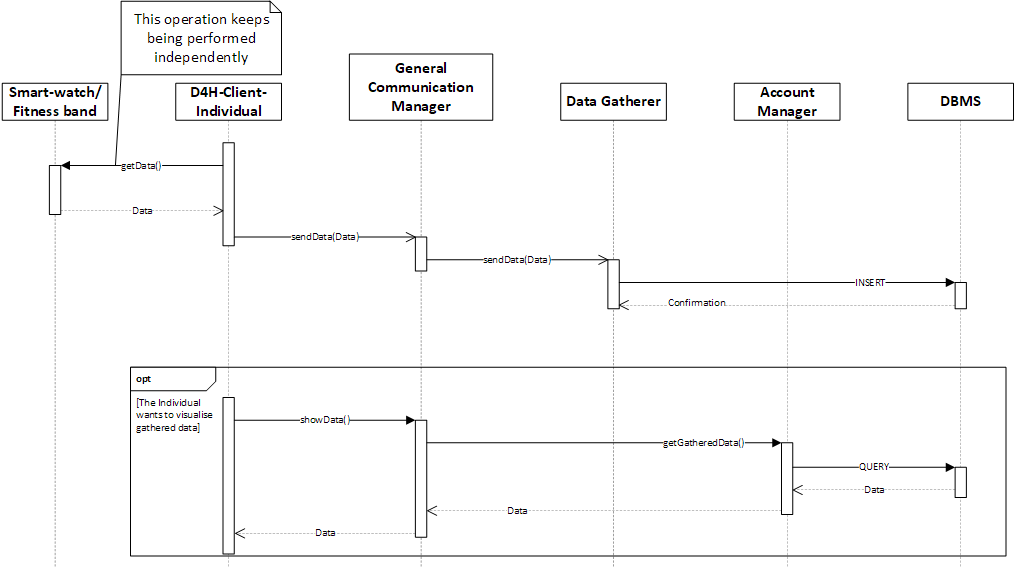
\includegraphics[scale=0.60]{pictures/DataCollection&Visualisation.png}}
    \caption{Data collection and visualisation sequence diagram}
    \label{fig:log&regDiagram}
\end{figure}

\subsubsection{Third Party Request History}
Thanks to the system a Third-party can visualise its old requests.
These kind of requests are taken by the Account Manager that provides to the Third-party all the history of the occurred requests.
Afterwards, if demanded, it provides also the details of each specific request, if the past request was accepted.

\begin{figure}[H]
    \centering
    \makebox[\textwidth][c]{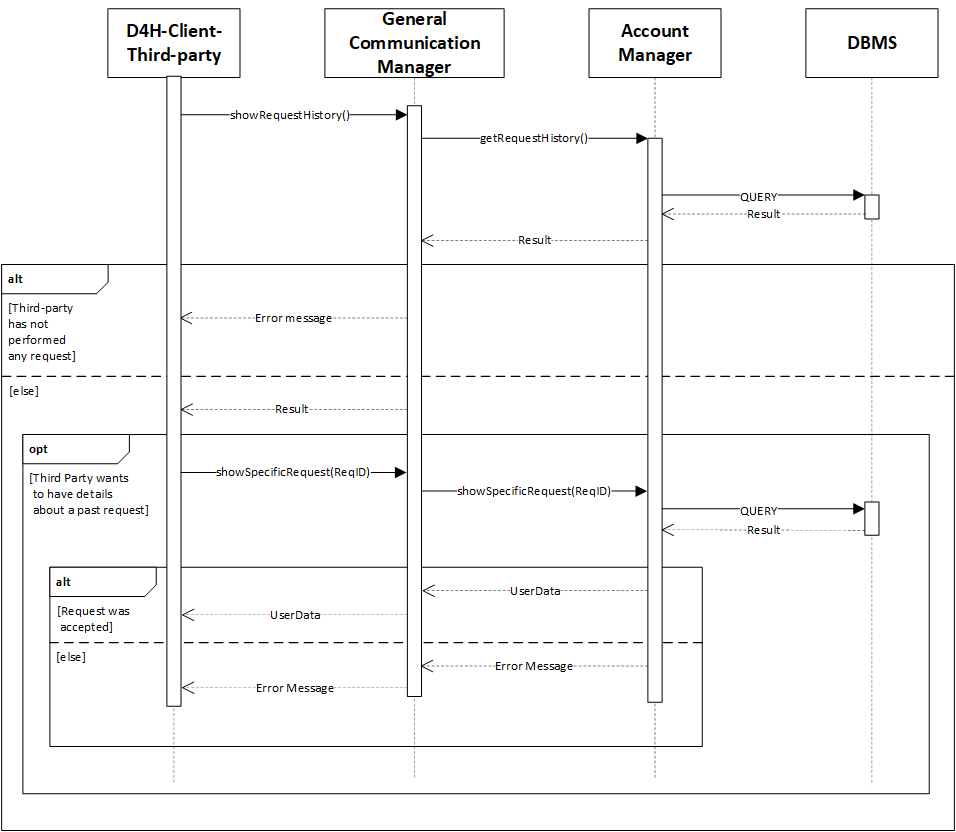
\includegraphics[scale=0.60]{pictures/ThirdPartyRequestHistory.png}}
    \caption{Third Party request history sequence diagram}
    \label{fig:log&regDiagram}
\end{figure}


\subsection{AutomatedSOS}

Concerning AutomatedSOS the only functionality highlighted is the ambulance dispatching.
AutomatedSOS interacts with Data4Help, collecting the users data needed to monitor the elderly people registered to it and interacting with the ambulance service in case of emergency.

\subsubsection{Subscription and Ambulance Dispatching}
First of all, an individual, that is already logged in Data4Help, needs to subscribe him/herself to the service. The system checks if his/her age matches with the bound imposed (65 years old), and then, it procedes to the subscription as follow. It makes a single request with subscription to D4H as a normal Third-party, the Individual receives the request with a notification coming from ASOS. After the acceptance, D4H starts to send data periodically to the Data Collector and Checker that analyses them and, in case of health parameters out of the thresholds set, calls the ambulance service, forwarding the position of the interested Elderly person.

\begin{figure}[H]
    \centering
    \makebox[\textwidth][c]{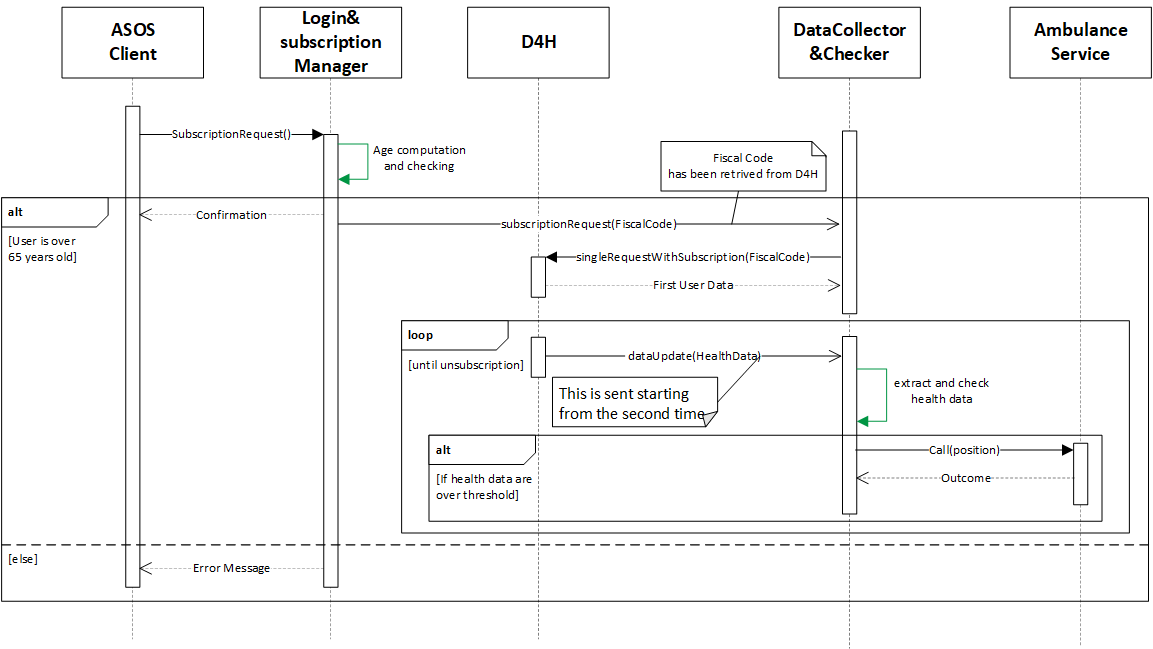
\includegraphics[scale=0.60]{pictures/AmbulanceDispatching.png}}
    \caption{Ambulance Dispatching sequence diagram}
    \label{fig:log&regDiagram}
\end{figure}

\subsection{Track4Run}
Concerning T4R the main functionalities touched are: The run organisation, the participants enrolment, the runners tracking and the ranking history requests.
Some of the others features have been already explained in the previous sections, for example the Organiser registration and log in is very similar to the log in and registration for a Third-party, with the only difference that the components are the ones of T4R.

\subsubsection{Run Organisation}
In the following diagram is explained how the system works to allow the Organiser to plan a run.
After the log in, the Organiser can make a new race request, handled by the Race Manager. It checks if there are other races at the same location at the same time, and after this verification, it contacts Google Maps. The latter is opened on the Organiser's device, in order to allow him/her to create the path desired, by adding manually on the Google Maps application each stop. Afterwards, when the path is defined the Organiser, through the T4R application, sends a notification to the Race Manager that stores the race details inside the database.

\begin{figure}[H]
    \centering
    \makebox[\textwidth][c]{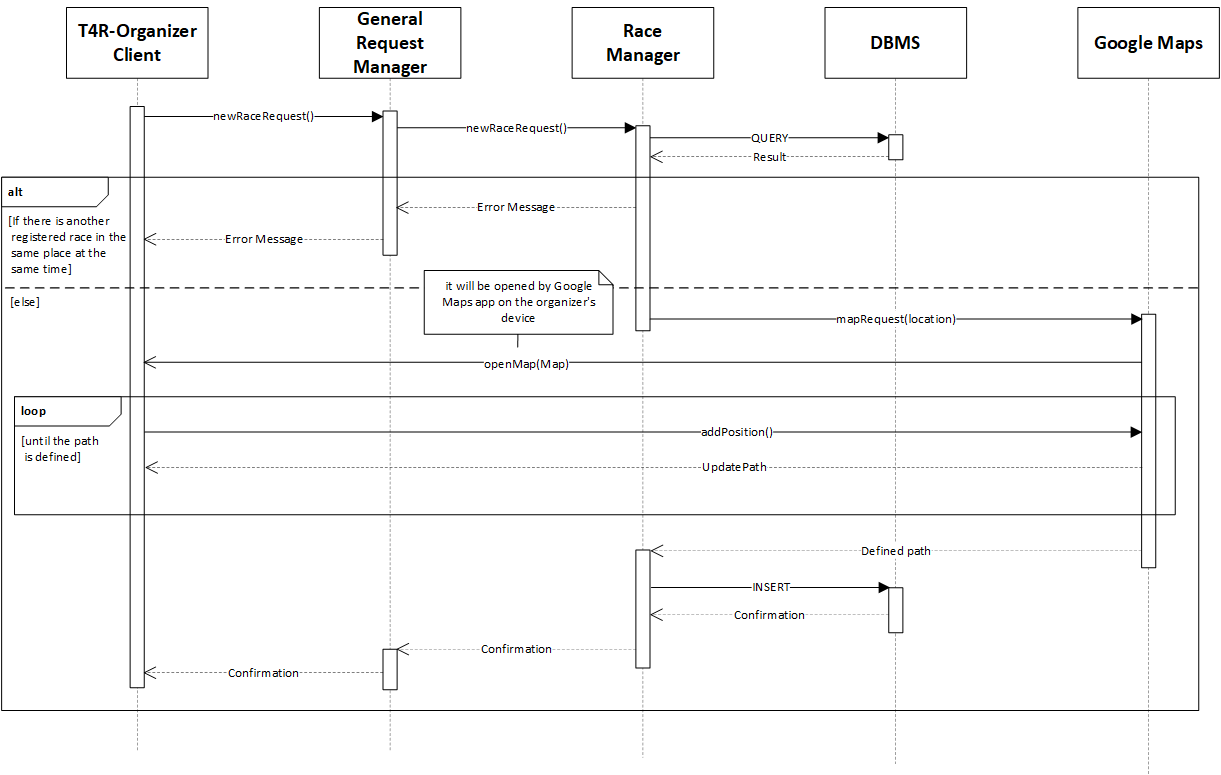
\includegraphics[scale=0.60]{pictures/RunOrganization.png}}
    \caption{Run organization sequence diagram}
    \label{fig:log&regDiagram}
\end{figure}

\subsubsection{Participant Enrolment}
After the race registration, any Data4Help Individual user can enrol to it.
The Race Manager receives the request from the General Request Manager, and checks if the Runner is enrolled to an other race at the same time. After this control, it verifies if the run already reached the maximum number of participants and, if it doesn't exceed, it adds the enrolling Participant.
In order to allow the Visitor to track the runner in a specific race, as will be explained in the next diagram, the General Request Manager, during the check-in of the runners, before the beginning of the race, sends a notification to the Tracker Manager that requests a single user subscription to Data4Help. The runner receives a request of subscription from T4R in his/her D4H application and, by accepting it, he/she confirms the participation to the race and the Tracker Manager starts to receive the data related to that Participant.

\begin{figure}[H]
    \centering
    \makebox[\textwidth][c]{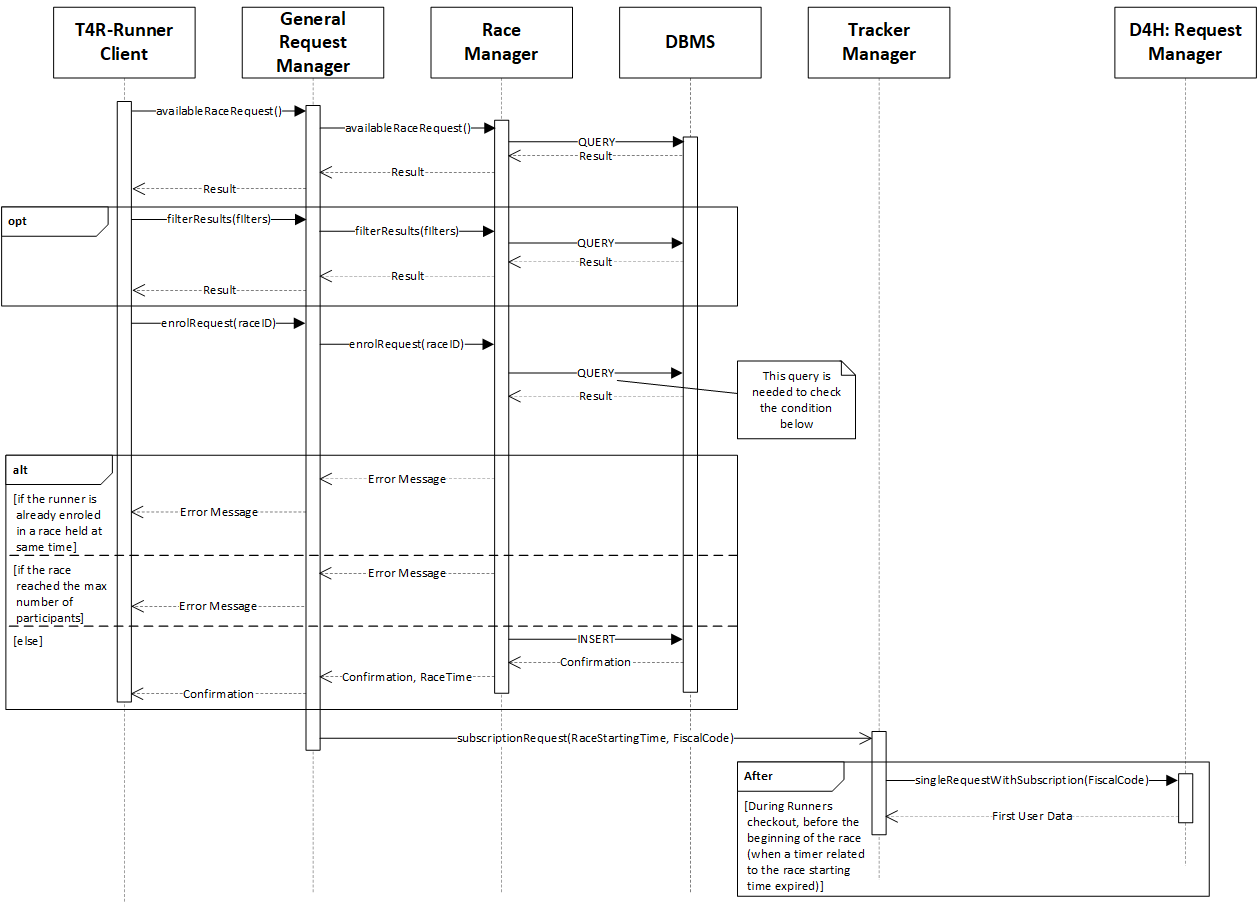
\includegraphics[scale=0.60]{pictures/ParticipantEnrollment.png}}
    \caption{Participant Enrolment sequence diagram}
    \label{fig:log&regDiagram}
\end{figure}

\subsubsection{Participant Tracking}
As described above, the spectator of a run, thanks to T4R, can track the participant during all the race.
They just have to download any application, Runner or Organiser edition, and without logging in they can enter in the tracking section.
Therefore, a Visitor can request the tracking for a specific race, this request passes through the General Request Manager and arrives to the Race Manager, that extracts all the Participants fiscal codes from the database, and sends them to the Tracker Manager. It filters the data received from D4H and, by sending the position to the Map service, it gets a map with the position of all the runners. This map is forwarded to the client periodically, in order to give the possibility to the Visitor to track all the participant at any time.

\begin{figure}[H]
    \centering
    \makebox[\textwidth][c]{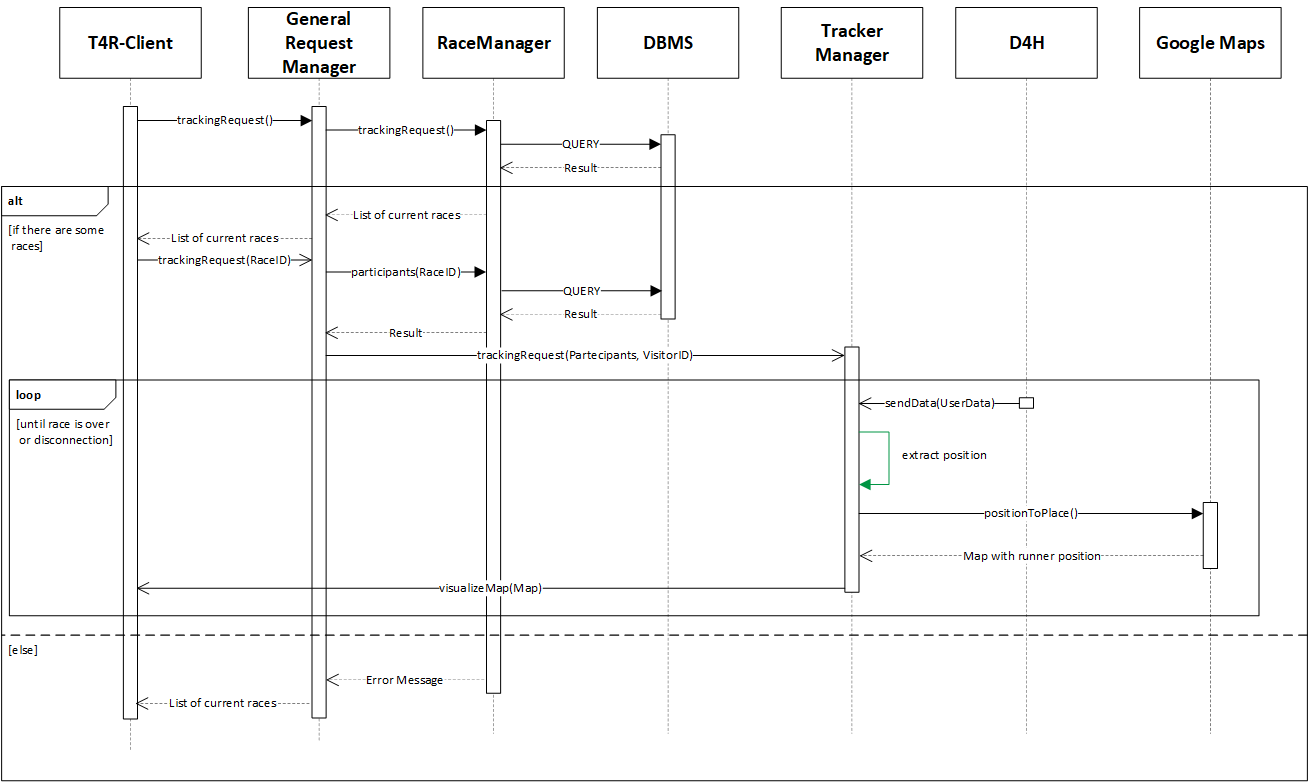
\includegraphics[scale=0.60]{pictures/ParticipantTracking.png}}
    \caption{Participant tracking sequence diagram}
    \label{fig:log&regDiagram}
\end{figure}

\subsubsection{Ranking History}
The last diagram shows the possibility of any client, both Organiser and Runner, to get the ranking of the past runs. The request is processed by the Account Manager that extracts the information from the database and returns them to the client.

\begin{figure}[H]
    \centering
    \makebox[\textwidth][c]{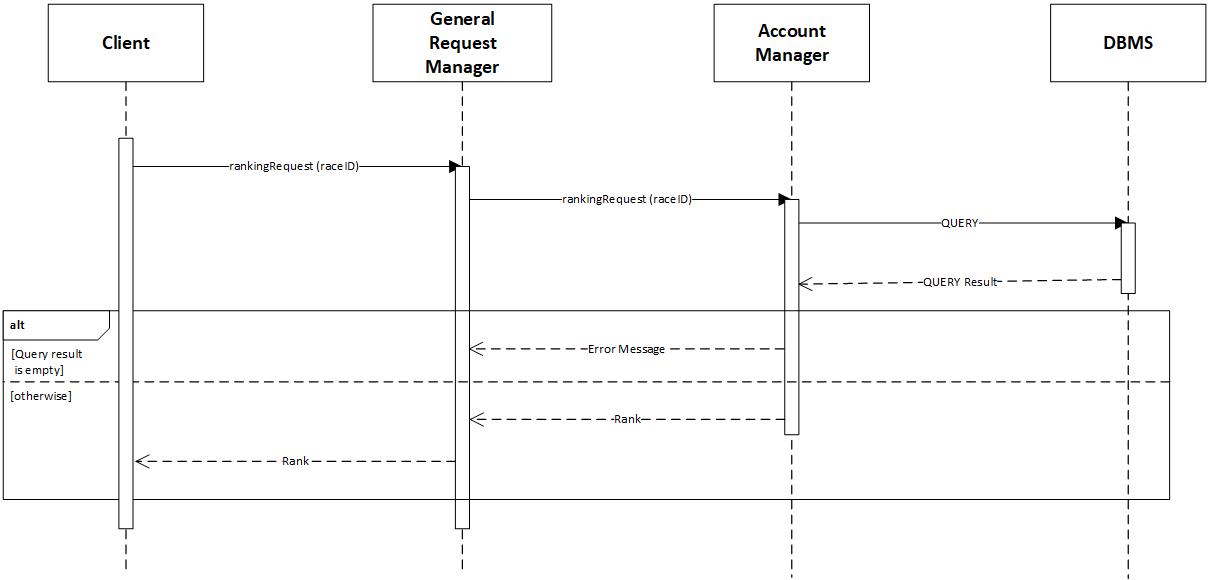
\includegraphics[scale=0.60]{pictures/RankingRequestSequenceDiagram.png}}
    \caption{Ranking history sequence diagram}
    \label{fig:log&regDiagram}
\end{figure}